%%%%%%%%%%%%%%%%%%%%%%%%%%%%%%%%%%%%%%%%%%%%%%%%%%%%%%%%%%%%%%%%%%%%%%%%%%%%%

\chapter{Context historique}

\section{La musique en Russie au début du XIX\ieme{} siècle}

Au début du XIX\ieme{} siècle, la Russie accuse un retard considérable pour ce qui est de la musique instumentale (symphonies, concertos, etc..). Cependant, c'est une période où le pays se transforme profondément. La société devient plus citadine et pratique d'avantage la musique occidentale.

En 1802, la \emph{société philharmonique de Saint Pétersbourg} est crée par des personnalités du monde de la culture, du monde de la finance, des musiciens et de riches aristocrates. La capitale découvre les œuvres peu connues de Mozart, Hayden et Beethoven. C'est ainsi, par exemple, que la \emph{Missa Solemnis} de Beethoven est donnée le 26 mars 1824 soit deux semaines avant la création viennoise.

Malgré les guerres napoléoniennes, la culture française demeure très appréciée par la haute société. Il en va de même pour la musique française et l'opéra italien. Rossini est découvert au cours des années 1820 et Verdi au cours des années 1840. Des musiciens tels que John Field (professeur de Mikhaïl Glinka) ou encore Anton Herke (professeur de Piotr Tchaïkovski ou Modeste Moussorgski) se chargeront de diffuser l'œuvres de Chopin ou Liszt. A partir des années 1840, les voyages en Russie s'intensifient avec la venue de Liszt, des époux Schumann, de Berlioz puis Wagner ultérieurement.

\section{La naissance de la musique russe}

À partir de 1783, Saint Pétersbourg se dote de son opéra : le \emph{Théâtre de Pierre}. Celui-ci sera succéssivement modernisé en 1802, 1818 et 1836. Comme la vie musicale s'intensifie, trois autres établissements sont construits : le \emph{Théâtre Alexandrinski} (1832), le \emph{Théâtre Mikhailovski} (1833) et le très célèbre \emph{Théâtre Mariinski} (1833).

Mais c'est avec les compositeurs Mikhaïl Glinka (1804-1857) et Alexandre Dargomyjski (1813-1869) que la Russie entame une nouvelle direction avec le développement d'une musique spécifiquement russe. Pour la première fois, il est fait emploi de matériaux historiques et traditionnels de façon réaliste. Le critique musical moderne Viktor Korchikov résume la situation ainsi : « On ne peut pas imaginer le développement de la culture musicale russe sans [...] les trois opéras : \emph{Ivan Soussanine} (Glinka, 1836), \emph{Rouslan et Ludmila} (Glinka, 1837-1842) et \emph{Le Convive de pierre} (Dargomyjski, 1866-1869) ».

Un autre tournant majeur consiste en la création, en 1858, de la \emph{Société Musicale Russe}. Sous l'impulsion d'Anton Rubinstein et sous le patronage de la grande-duchesse Elena Pavlovna, sa mission est de répendre l'enseignement de la musique classique et contemporaine au sein de l'empire. La \emph{Société Musicale Russe} gagne très rapidement en professionalisme. Avec le soutien du prince Nikolaï Troubetskoï, Nicolaï Rubinstein, le frère de d'Anton Rubinstein et grand ami de Piotr Tchaïkovski, devient président \emph{Société Musicale de Moscou}. La création des concervatoires de Saint Pétersbourg (1862) puis de Moucou (1866) compte parmi les plus grandes réussites. Dés lors, la croissance est fulgurante, la \emph{Société Musicale Russe} s'installe à Kiev (1861), à Kazan (1864), à Kharkov (1871), à Nijni Novgorod (1873?), etc... Juste avant la révolution de 1917, date de la dissolution et la \emph{Société Musicale Russe}, une cinquantaine de filiales sont disséminées dans tout l'empire. 

\section{Le groupe des cinq}

Les guerres napoléoniennes ont entrainé une prise de conscience nationale et l'émmergeance d'un patriotisme officialisé sous le règne de Nicolas I\ier{} (1825-1855).  Sous Alexandre II (1855-1881) puis Alexandre III (1881-1894), les conditions plus libérales sont optimales pour le développement de la \emph{Société Musicale Russe}, mais aussi pour le développement du fameux \emph{Groupe des Cinq}.

Le \emph{Groupe des Cinq} est le cercle de musiciens plus ou moins autodidactes fédéré par Mili Balakirev (chef d'orchestre empirique, 1837-1910) à partir de 1857. César Cui (ingénieur en fortifications, 1835-1918) et Modeste Moussorgski (officier, 1839-1881) furent les premiers à rejoindre le groupe suivis par Nicolaï Rimski-Korsakov (élève officier de marine, 1844-1908) en 1861 puis enfin Alexandre Borodine (médecin et chimiste, 1833-1887) en 1862.

Le goupe défend l'idéal d'une musique spécifiquement russe (folklore national, orientalisme), sur le modèle de Mikhaïl Glinka, libérée de la tutelle des écoles italienne ou allemande. Il est réfractère aux frères Rubinstein mais promouvoit la musique romantique moderne (Berlioz, Chopin, Liszt, Schumann) plus novatrice et peu encore diffusée en Russie. En 1868, Piotr Tchaïkovski, qui entretient de bonnes relations avec Mili Balakirev et Nicolaï Rimski-Korsakov, espère devenir le sixième membre du groupe. L'éloignement géographique - Tchaïkovski enseigne au conservatoire de Moscou, le \emph{Groupe des Cinq} est basé à Saint Pétersbourg - et le cosmopolitisme de Tchaïkovski interdiront ce rapprochement. À partir de 1872, la réussite et la « traîtrise » de Rimski-Korsakov, l'échec persistant de Cui et la mort de Moussorgski et Borodine auront raison du cénacle.

Le \emph{Groupe des Cinq} laisse une production musicale importante\footnote{\emph{Islamey} et \emph{Tamara} pour Balakirev, \emph{Le Prince Igor} et \emph{Dans les steppes de l'Asie centrale} pour Borodine, \emph{Une nuit sur le mont Chauve}, \emph{Boris Godounov} et \emph{Tableaux d'une exposition} pour Moussorgski, \emph{Shéhérazade}, \emph{Capriccio espagnol} et \emph{Le Coq d'or} pour Rimski-Korsakov, ...} et jouit d'une importance de premier ordre dans l'histoire de la musique russe et européenne.

Une dizaine d'années après la dissolution du groupe des \emph{Groupe des Cinq}, Balakirev forme un second cercle de musiciens\footnote{D'autres groupes ont existé, citons par exemple le \emph{cercle Belyayev} de Saint Petersburg (1885-1908) avec Nikolai Rimsky-Korsakov, Alexander Glazunov, Vladimir Stasov, Anatoly Lyadov, Alexander Ossovsky, Witold Maliszewski, Nikolai Tcherepnin, Nikolay Sokolov, Alexander Winkler, etc... } dont le membre le plus éminent n'est autre que Sergueï Liapounov. Ce mémoire étant dédié à l'étude de l'œuvre de ce dernier, le rapport entre les deux homme sera plus extensivement discuté dans les chapitres suivants. La figure \ref{frise} récapitule la chronologie des principaux événements depuis la naissance de Mikhaïl Glinka jusqu'à la mort de Sergueï Liapounov.

\begin{figure}[!ht]
  \begin{bigcenter}
    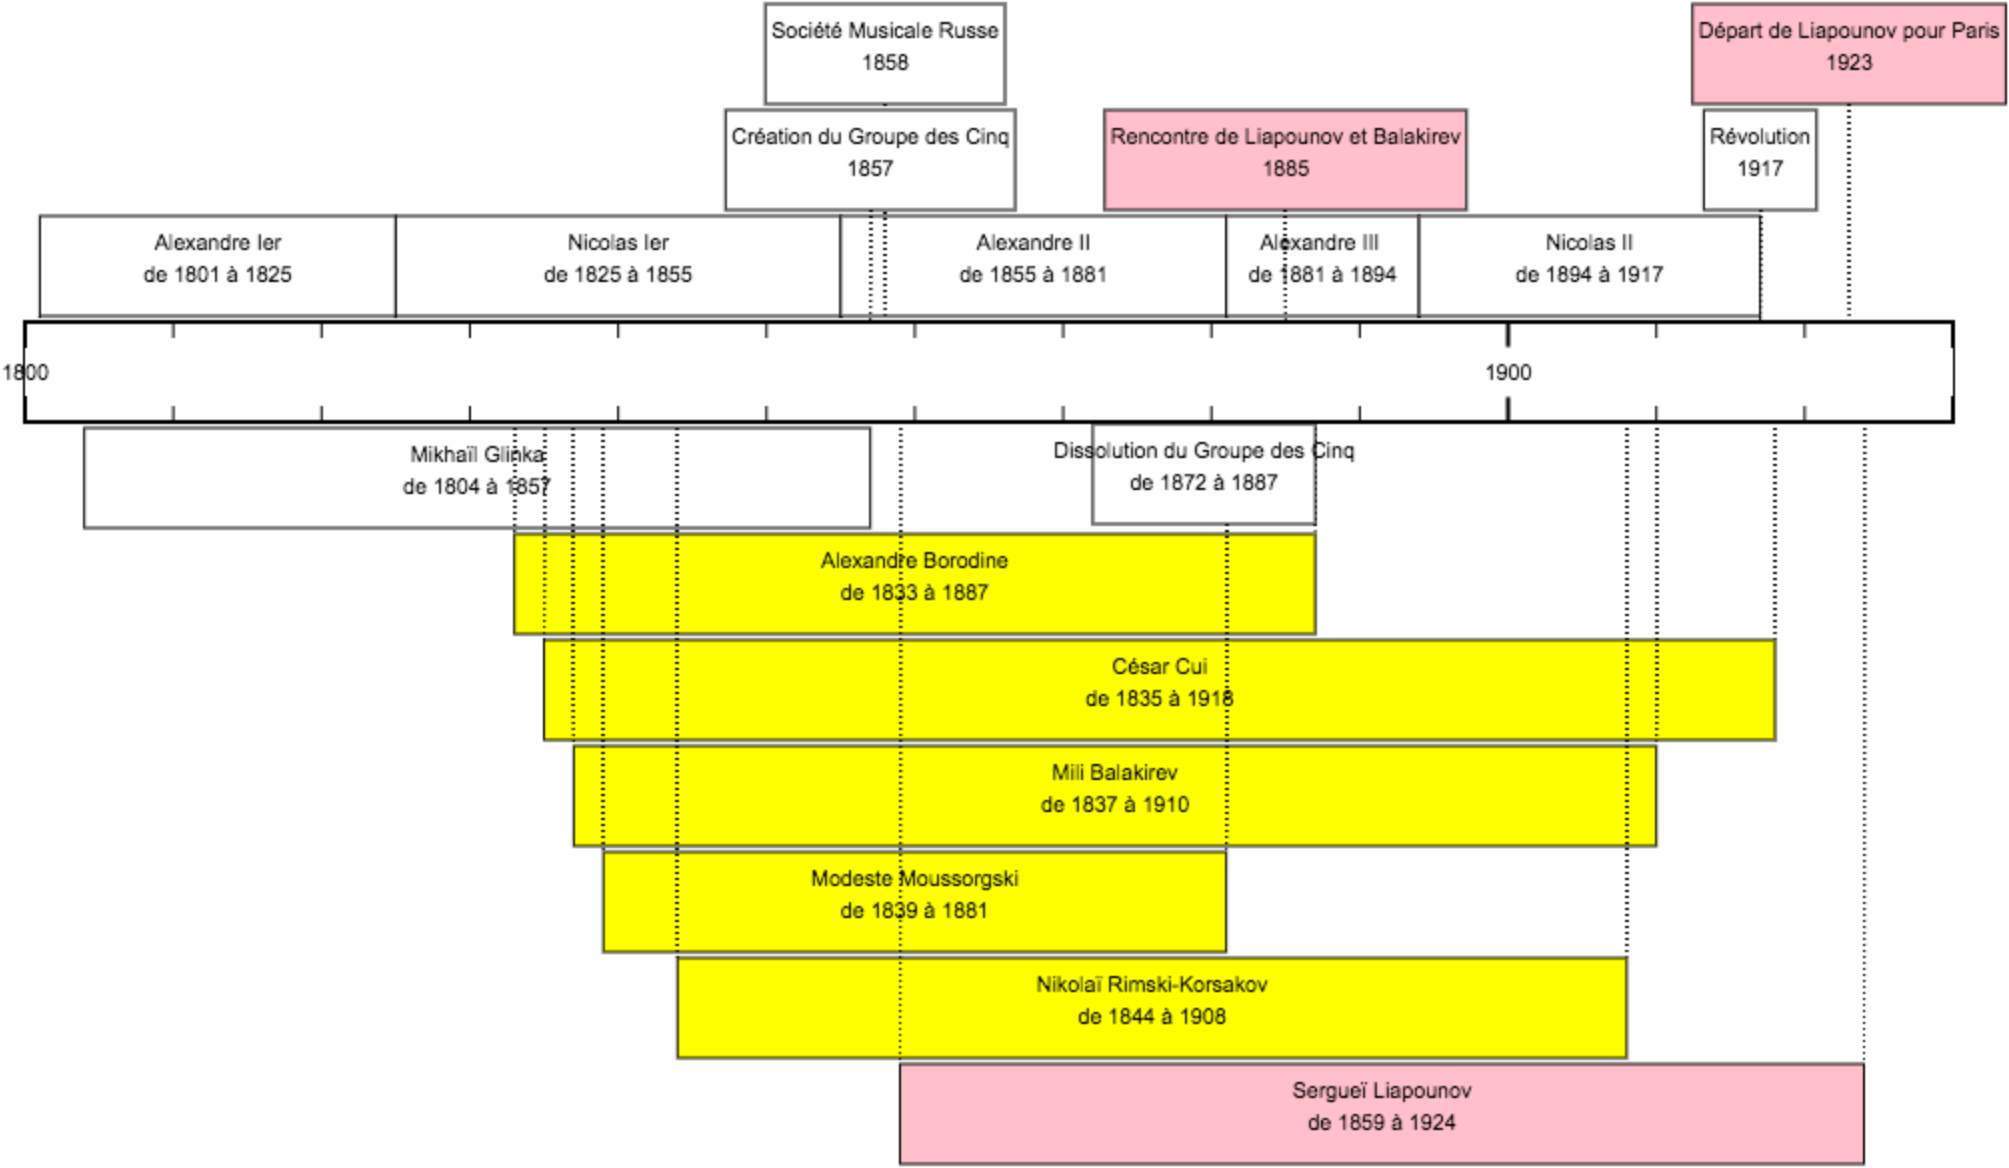
\includegraphics[width=15.5cm, keepaspectratio]{frise.png}
  \end{bigcenter}
  \caption{\label{frise}Frise chronologique des principaux événements depuis la naissance de Mikhaïl Glinka jusqu'à la mort de Sergueï Liapounov.}
\end{figure}

%%%%%%%%%%%%%%%%%%%%%%%%%%%%%%%%%%%%%%%%%%%%%%%%%%%%%%%%%%%%%%%%%%%%%%%%%%%%%

\chapter{L'œuvre de Sergueï Liapounov}

Ce chapitre est dédié à l'étude de la bibliographie et de l'œuvre Sergueï Liapounov. Plus particulière nous essayerons de positionner ce dernier face aux héritages du romantisme européen et face à l'idéal musical du groupe \emph{Groupe des Cinq}. Nous nous intéresserons plus particulièrement aux \emph{12 études d'execution transcendante} qui sont typiquement russes de par leur couleurs slaves mais s'inscrivent dans la continuité des études éponymes de Franz Liszt. Finallement, nous essayerons de dégager les principales raisons de l'anonymat de ce compositeur qui semble pourtant laisser une marque importante dans l'histoire de la culture musicale russe\ref{onegina1}.

\section{La jeunesse du compositeur}

Sergueï Mikhaïlovitch Liapounov (ou Lyapunov) est un compositeur, pianiste virtuose, chef d'orchestre, éthnomusicologue, éditeur et pédagogue russe, né le 30 novembre 1859 à Iaroslavl\footnote{Iaroslavl est la capitale administrative de l'oblast de Iaroslavl. La ville est située au confluent de la Volga et de la Kotorosl, à 282 km au nord-est de Moscou.} et mort le 8 novembre 1924 à Paris. Son père, l'astronome Mikhail Vassilievitch Liapounov et sa mère Sofia Aleksandrovna Shilipova ont eu trois fils. L'aîné Alexandre Liapounov (1857-1918) est un célèbre mathématicien connu pour ses travaux sur l'étude des systèmes dynamiques (stabilité au sens de Liapounov). Le cadet Boris Lyapunov (1862–1943) est un linguiste spécialisé dans les langues slaves et membre de l'\emph{Académie des Sciences}.

Le talent musical de Liapounov se manifeste très tôt. Encore incapable de parler, il réclame le piano. Âgé de quatre ans et accompagné de son fère Alexandre, il reçoit ses premiers cour de piano de sa mère, une femme instruite un bonne pianiste. Après la mort prématurée du père en 1868, la famille Liapounov s'installe à Nijni Novgorod\footnote{Nijni Novgorod est capitale administrative de l'oblast de Nijni Novgorod et centre économique de la région économique de Volga-Viatka. La ville est située au confluent de la Volga et de l'Oka, à 405 km à l'est de Moscou.}. Liapounov prend des cours de piano par l'intermédiaire de l'antenne de Nijni Novgorod de la \emph{Société Musicale Russe}. A cette époque, il s'implique dans des conserts étudiant et interprète publiquement des œuvre de Bach, Haydn, Beethoven et Mendelssohn. A la fin de ses études et sur les recommandations de Nikolaï Rubinstein lui même, il s'inscrit en 1878 au conservatoire de Moscou. Ses principaux professeurs sont Karl Klindworth et Paul Pabst (deux anciens élèves de Franz Liszt) pour le piano et Sergueï Taneïev et Piotr Tchaïkovski pour la composition.

En 1883, lorsque Liapounov termine ses études, il est devenu un véritable virtuose\footnote{Sa fille, Anastasia Liapounov, a laissé une des rares descriptions sur le jeu pianistique de son père : « ... la simplicité du phrasé avec une variété considérable de sonorités. Son jeu était simple, noble, calme, peut-être même trop équilibré .... ».}. Son catalogue d'œuvres jouées est important et compte des pièces de difficultés considérables. A titre d'exemple, on peut citer les concertos de Chopin ou encore le diabolique \emph{Islamey} de Balakirev. Cependant, il ne se destine pas à une carrière de concertiste. De ses aveux même, il ne se concidère pas comme un pianiste majeur, le jeune pianiste manque de confiance en lui sur scène. Il refuse le post d'enseignant offert par Nikolaï Rubinstei estimant que « la vraie route qui doit passer par la musique russe ». En effet, il développe un sentiment de rejet à l'égare de l'école de Moscou et de Tchaïkovski. C'est à ce moment qu'il rencontre Mili Balakirev pour la première fois. Le jeune compositeur prend la décision ferme d'adhérer au \emph{Groupe des Cinq}. En 1885, il s'établi à Saint Pétersbourg.

C'est durant les années 1880 que Liapounov compose ses prémières œuvres sérieuses. L'influence de la musique de Chopin et Liszt est très marquée. A titre d'exemple, citons la valse op. 1 (voir figure \ref{op1}) ou encore \emph{Rêverie du soir}, op. 3 (voir figure \ref{op3}) où il est intéressant de noter la couleur orientable des premières mesures. Le nocturne op. 8, écrit quelques années plus tard, est un très bel hommage à la musique de Chopin.

\begin{figure}[!ht]
  \begin{bigcenter}
    \begin{tabular}{lr}
      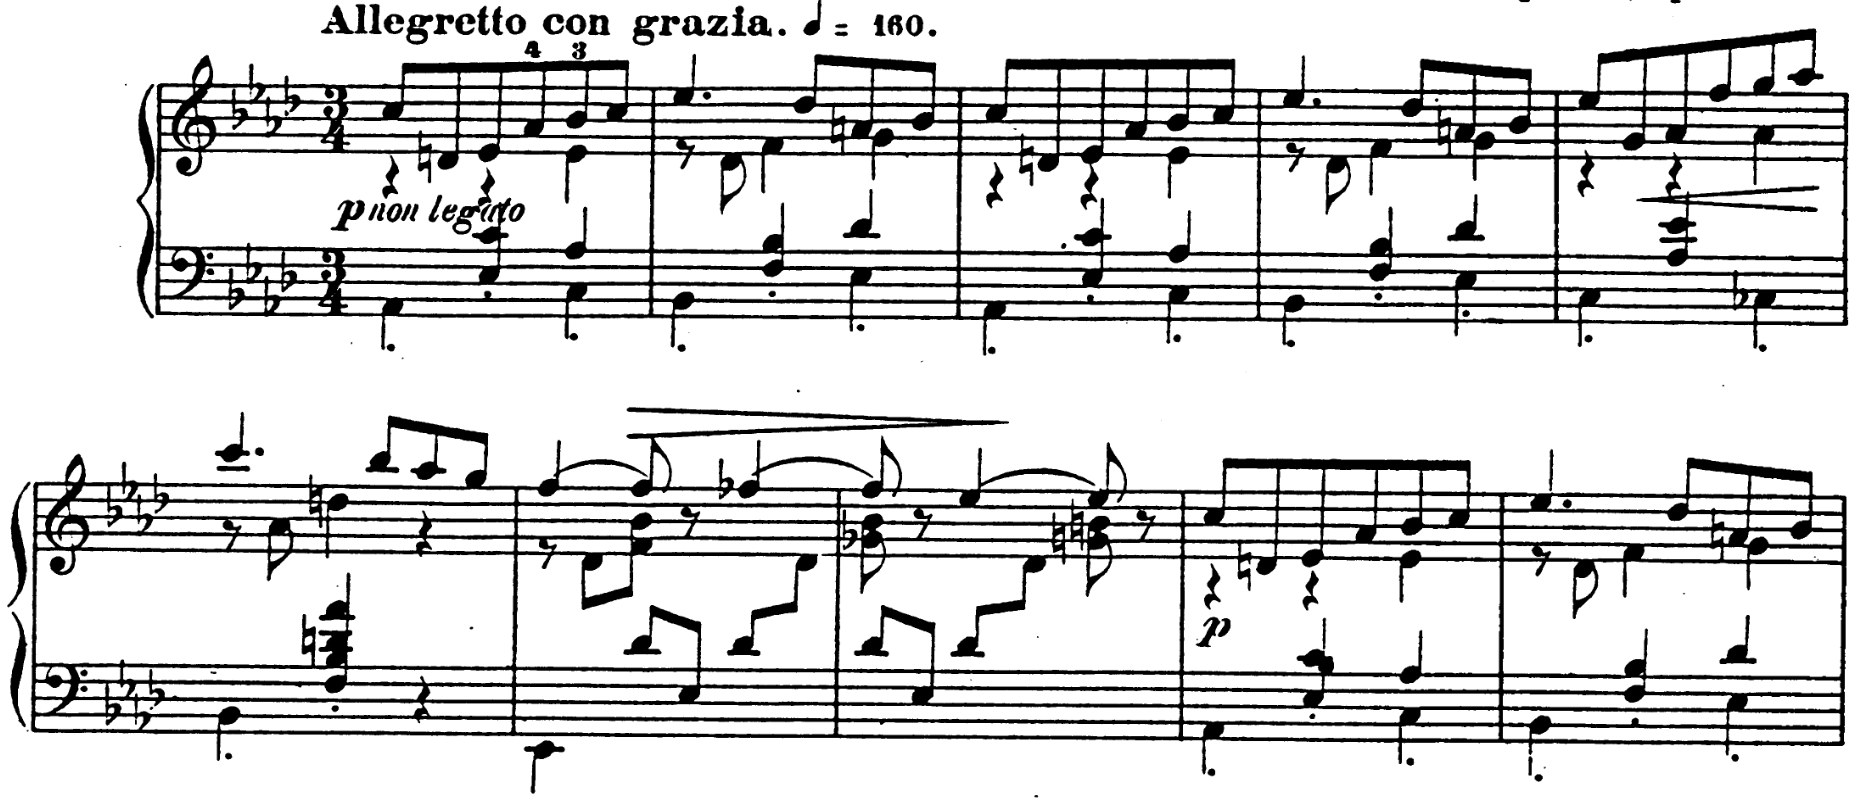
\includegraphics[width=12.5cm, keepaspectratio]{op1.png}
      &
      
\includegraphics[width=3cm, keepaspectratio]{op1-qr.png}
    \end{tabular}
  \end{bigcenter}
  \caption{\label{op1}Extrait de \emph{Trois Morceaux} op. 1 n\degre 3 : Valse.}
\end{figure}

\begin{figure}[!ht]
  \begin{bigcenter}
    \begin{tabular}{lr}
      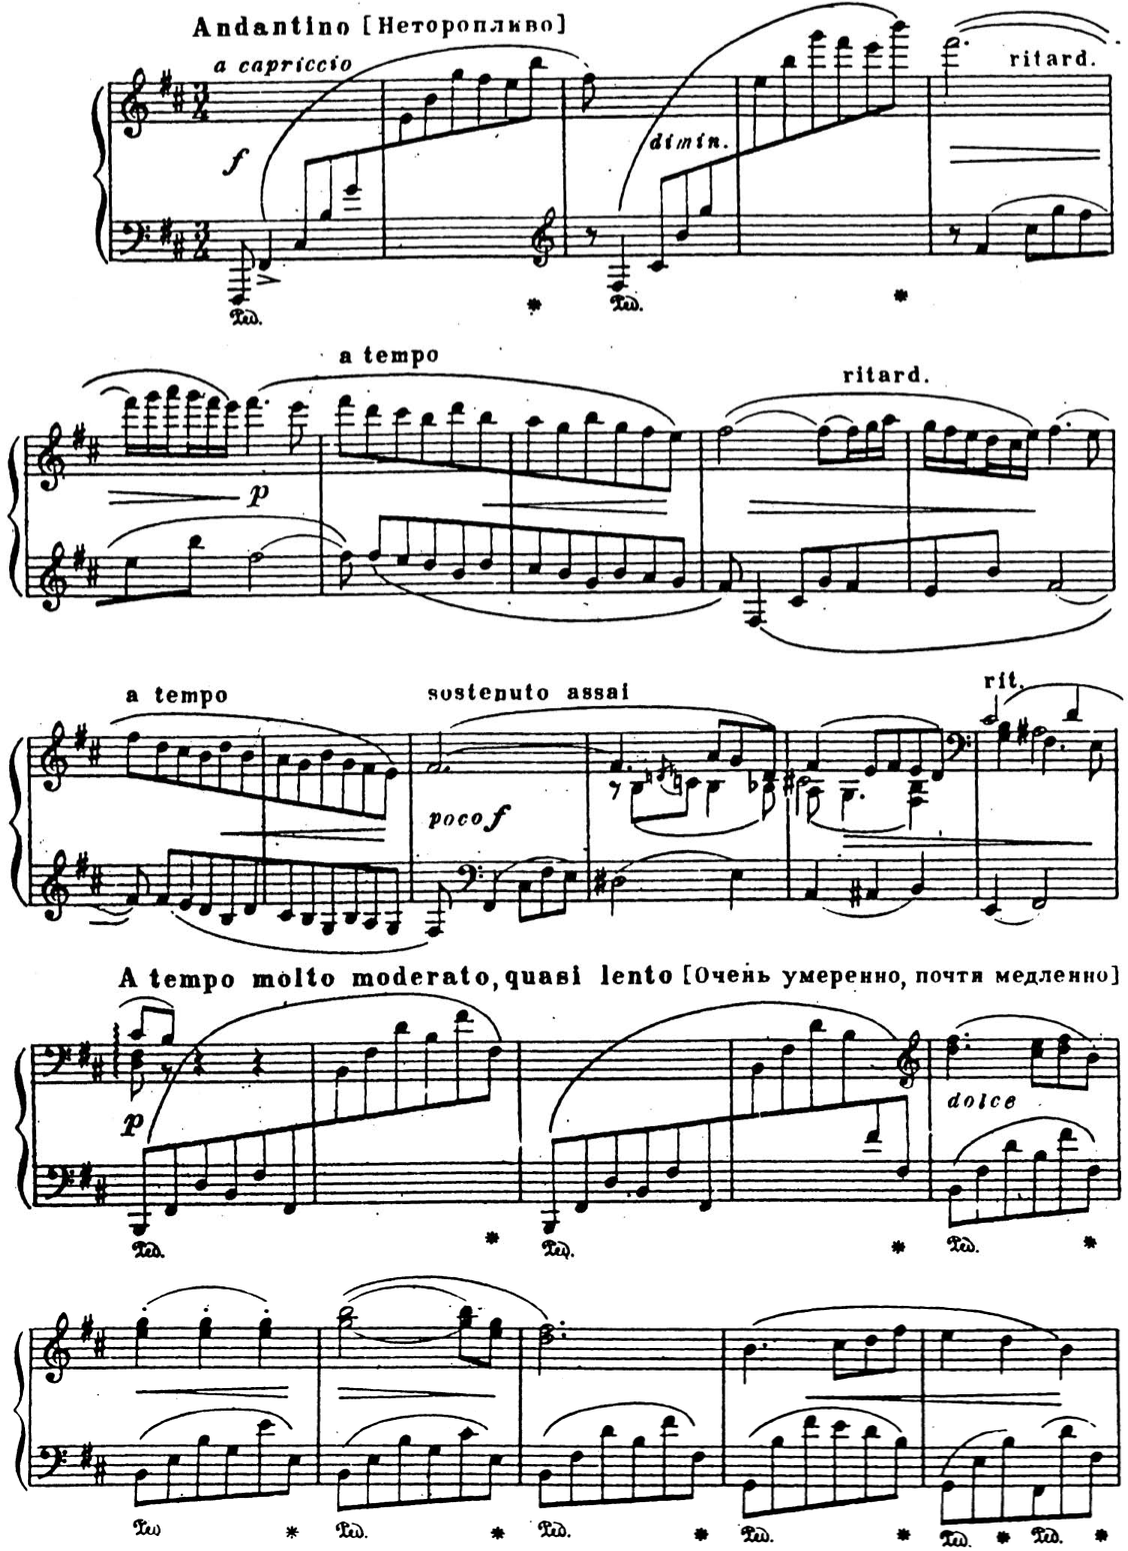
\includegraphics[width=12.5cm, keepaspectratio]{op3.png}
      &
      
\includegraphics[width=3cm, keepaspectratio]{op3-qr.png}
    \end{tabular}
  \end{bigcenter}
  \caption{\label{op3}Extrait de \emph{Rêverie du soir} op. 3.}
\end{figure}

\begin{figure}[!ht]
  \begin{bigcenter}
    \begin{tabular}{lr}
      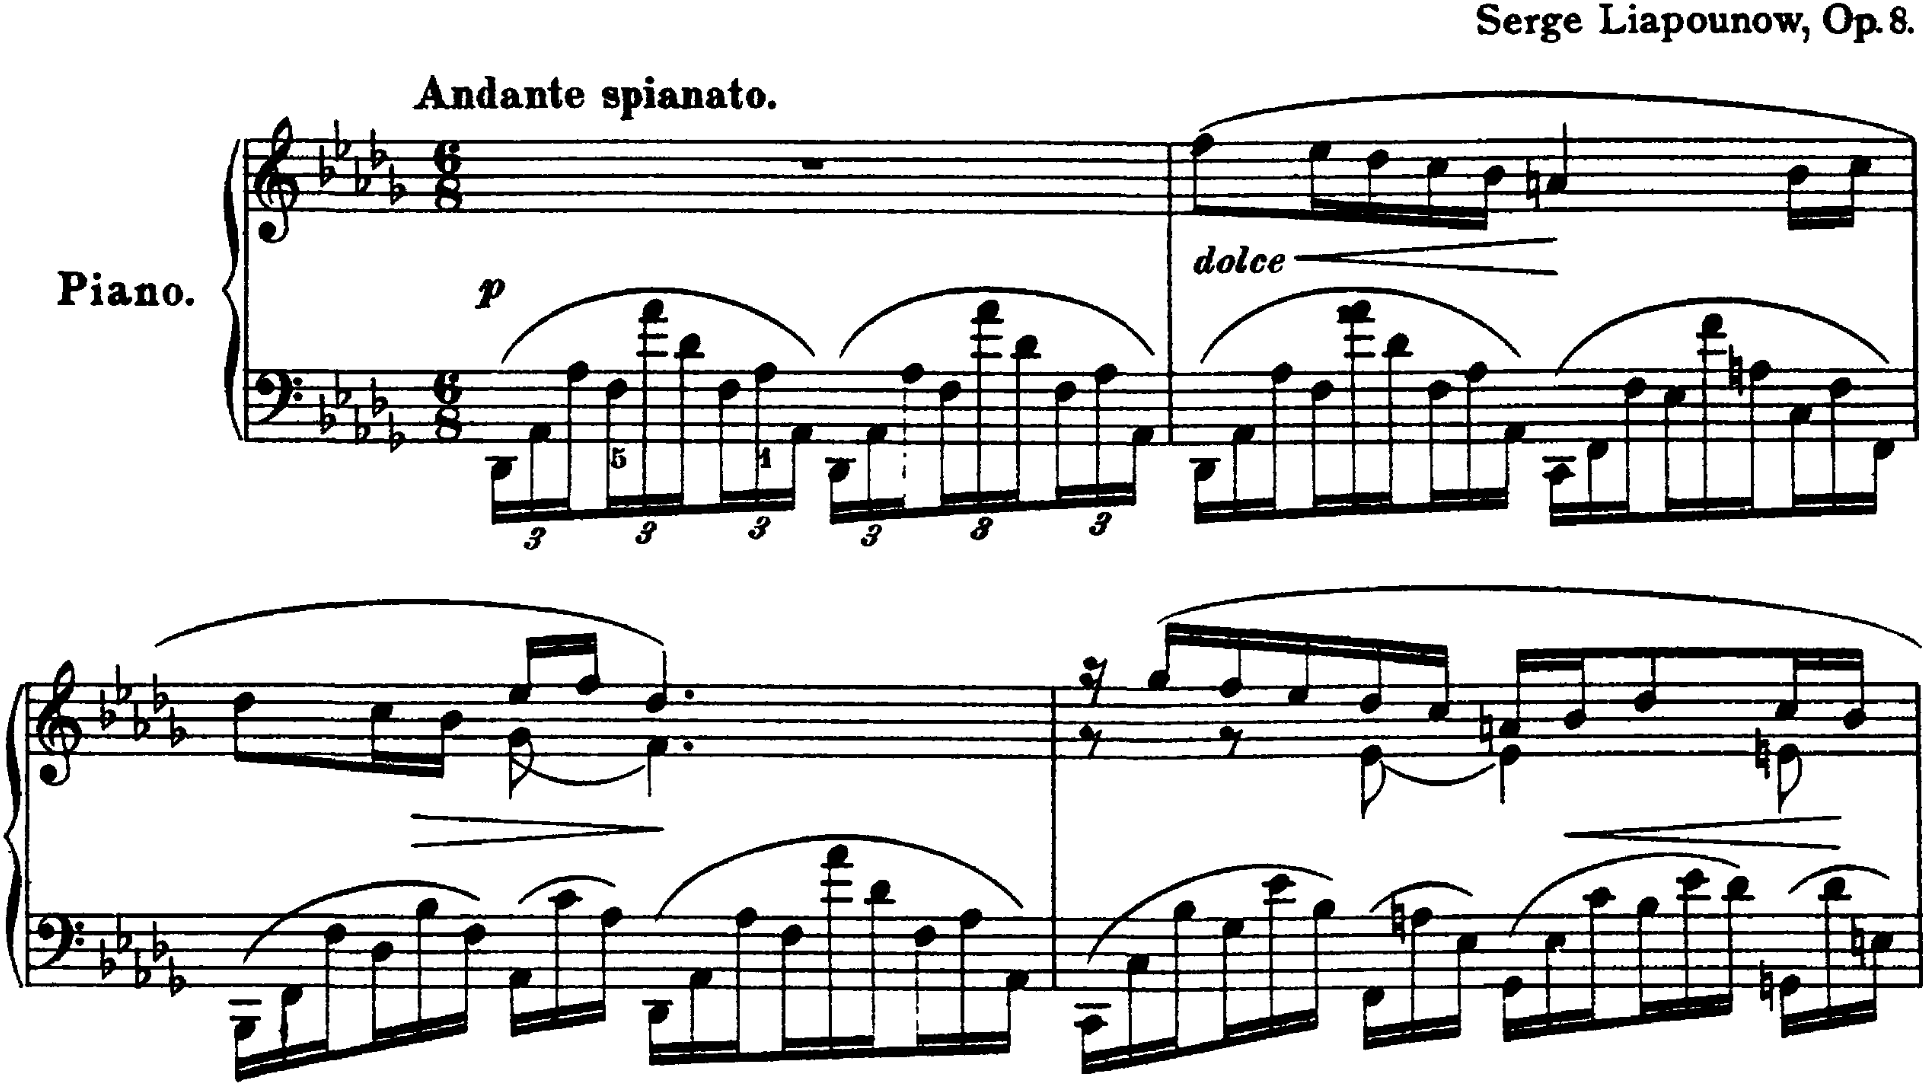
\includegraphics[width=12.5cm, keepaspectratio]{op8.png}
      &
      
\includegraphics[width=3cm, keepaspectratio]{op8-qr.png}
    \end{tabular}
  \end{bigcenter}
  \caption{\label{op3}Extrait de \emph{Nocture} op. 8.}
\end{figure}

\section{Liapounov et Balakirev}

TODO

\section{Les \emph{12 études d'execution transcendante} op. 11}

%%%%%%%%%%%%%%%%%%%%%%%%%%%%%%%%%%%%%%%%%%%%%%%%%%%%%%%%%%%%%%%%%%%%%%%%%%%%%

\chapter{Conclusion}

%%%%%%%%%%%%%%%%%%%%%%%%%%%%%%%%%%%%%%%%%%%%%%%%%%%%%%%%%%%%%%%%%%%%%%%%%%%%%
